\chapter{Physics of Z Transverse Momentum}
\label{chapter:theory}

\section{The Standard Model}
\label{section:standard_model}

Our current understanding of how matter interacts at high energy is entirely
described by the standard model (SM) as constructed by Weinberg, Glashow, and
Salam \cite{glashow1961}\cite{weinberg1967}\cite{salam1968}. The model combines
three of the four fundamental forces (leaving out only gravity, which is so
weak as to be negligible) and explains almost everything we see in the
universe.

\subsection{The Electromagnetic Force}
\label{subsection:electronmagnetic_force}

The modern theory of electromagnetism began with Maxwell's theory developed in
the middle of the 19th century \cite{maxwell1863}. Maxwell was the first to
conclude that light was an electromagnetic wave, the full importance of which
was only later understood when it was discovered that the photon was the force
carrier of the electromagnetic force \cite{maxwell1865}.

In the early 20th century, Lorentz and Einstein developed relativistic
mechanics and showed that Maxwell's theory was Lorentz invariant
\cite{lorentz1899}\cite{einstein1904}. Dirac updated the theory in 1920 when he
was able to quantize the electromagnetic field as an ensemble of harmonic
oscillators \cite{dirac1927}. Dirac would go on to discover that anti-particles
were a natural consequences of his equations \cite{dirac1928}\cite{dirac1930}.
These anti-particles were found by Anderson in 1932 as he observed cosmic rays
in a cloud chamber \cite{anderson1933}.

As microwave technology improved in the 1940s, more accurate measurements of
the energy level shifts in hydrogen were made, resulting in the discovery of
the Lamb shift by Lamb and Rutherford \cite{lamb1947}. This discovery pointed
to discrepancies in the theory, discrepancies which Bethe would explain after
completing a set of non-relativistic calculations using it \cite{bethe1947}.
Bethe's work inspired multiple other physicist including Dyson, Feynman,
Schwinger, and Tomonaga to work along similar lines. They created quantum
electrodynamics, a fully relativistic and self-consistent theory of
electromagnetic interactions
\cite{tomonaga1946}\cite{schwinger1948}\cite{feynman1949}\cite{dyson1949}.

\subsection{The Weak Force}
\label{subsection:weak_force}

The need for a weak force, and hence a theory describing it, was first hinted
at by beta decay experiments in the early 1900s. These experiments culminated,
in 1914, in Chadwick's discovery that the energy spectrum of electrons ejected
in beta decay was continuous instead of a delta function as would be expected
for a two-body decay \cite{chadwick1914}. While some proposed that this
discovery indicated that momentum and energy were not conserved, Pauli proposed
an alternative: there was a neutral and invisible particle that carried away
some of the energy---the neutrino \cite{pauli1930}. Fermi began working on this
idea and invented a four fermion contact interaction in which a neutron decayed
into a proton, an electron, and a neutrino \cite{fermi1934}.

In 1947, Rochester and Butler discovered a particle that decayed to two pions
which they called the $\theta$; in 1949, Brown and Powell discovered a particle
that decayed to three pions which they called the $\tau$
\cite{Rochester1947}\cite{brown1949}. It was soon discovered that these
particles had the same mass and lifetime---indicating that they were the same
particle---but, based on their decay products, they must have different parity.
Lee and Yang proposed that there was only one particle undergoing a parity
violating decay \cite{lee1956}. Their idea was confirmed by Wu in 1956, who
showed that electrons were preferential emitted from \cobaltsixty in one
direction, and by Garwin, Lederman, and Weinrich in 1957, who studied \pitomunu
in a storage ring \cite{wu1956}\cite{garwin1957}.

In 1954, Yang and Mills replaced Fermi's contact interaction with a non-Abelian
gauge theory that contained a spin-1 boson to mediate the force
\cite{yang1954}. However, this boson was massless, and so the weak force's
range would have been invite. In 1960, Glashow was able to modify Yang and
Mill's theory by adding Sudarshan and Marshak's vector minus axial ($V-A$)
model to produce a unified electroweak force described by the \SUtwoUone gauge
group \cite{glashow1961}\cite{sudarshan1958}. \SUtwo is a left-handed
interaction and so violates parity as expected. Weinberg and Salamn finished up
the model in 1967 when they added the Brout, Englert, and Higgs mechanism which
made the vector bosons mass and so explained the short ranged nature of the
weak interaction
\cite{weinberg1967}\cite{salam1968}\cite{englert1964}\cite{higgs1964}.

\subsection{The Strong Force}
\label{subsection:Strong_force}

The theory of the strong force grew out of studies of atomic nuclei. In 1911,
Rutherford discovered that that atomic nucleus was a compact, positively
charged object \cite{rutherford1911}. 1917, Rutherford showed that larger
nuclei were composed of hydrogen nuclei and so discovered the proton
\cite{rutherford1919}. The discovery of the uncharged neutron in 1932 by
Chadwick indicated that the atomic nucleus was made up of multiple types of
nucleons, and that it could not be held together by the electromagnetic force
\cite{chadwick1932}. In 1934, Yukawa---having noted that Fermi's contact
interaction was too weak to hold nuclei together---tried to explain this
nuclear force using meson exchange \cite{yukawa1935}. In 1947, Lettes,
Occhialini, and Powell discovered the pion which seemed to confirm Yukawa's
theory \cite{lattes1947}.

In the 1950s and early 1960s, dozens of new mesons were discovered, indicating
the need for a new theory. Some of these new mesons seemed to have a new type
of quantum number that limited their available decays, leading them to be
called ``strange'' particles. An effort to explain these particles lead to the
Gell-Mann--Nishijima formula
\cite{nakano1953}\cite{nishijima1955}\cite{gellmann1956}. This theory lead
Gell-Mann and Ne'eman to come up with a classification scheme for mesons and
baryons based on the \SUthree which Gell-Mann named the Eightfold Way. In 1964,
Gell-Mann and Zweig realized that the Eightfold Way implied that mesons were
composed of sub-atomic particles which became known as quarks
\cite{gellmann1964}\cite{zweig1964}. This model was used to predict the
existence of the charm quark, and upon its success was incorporated with
electroweak theory to form the full \SUthreeSUtwoUone symmetry group of the
standard model.

\subsection{Experimental Verification}

The standard model has has made numerous predictions which have been borne out
by experiment. The neutral current interaction was observed by the Gargemelle
experiment at CERN in 1973 shortly after it was predicted by Weinberg, Glashow,
and Salam \cite{hasert1973}. This confirmation of their theory won the trio the
Nobel Prize in 1979. The remaining quarks were found over the next twenty
years. The charm was found at SLC and BNL in 1974 via \jpsi decays
\cite{aubert1974}\cite{augustin1974}. The bottom was discovered at FNAL in 1977
by the E288 experiment \cite{herb1977}. The final quark, the incredibly heavy
top, had to wait until 1995 to be discovered by the CDF and D0 experiments
running at the Tevatron at FNAL \cite{cdf1995}\cite{d01995}. The \W and \Z
bosons were discovered at CERN in 1983 at the UA1 and UA2 experiments running
Super Proton Synchrotron \cite{ua1_w}\cite{ua2_w}\cite{ua1_z}\cite{ua2_z}.
These bosons were an excellent test of the standard model as their masses could
be very exactly calculated. The discovered bosons matched the calculated masses
to high precision. The final piece of the standard model, the Higgs bosons, was
discovered by ATLAS and CMS in 2012 using the LHC at CERN
\cite{atlas_higgs}\cite{cms_higgs}. Although precession measurements of the
Higgs are still ongoing, it so far precisely matches the predictions of the
standard model.

\subsection{Components of the Standard Model}

\begin{figure}[tb]
    \centering
    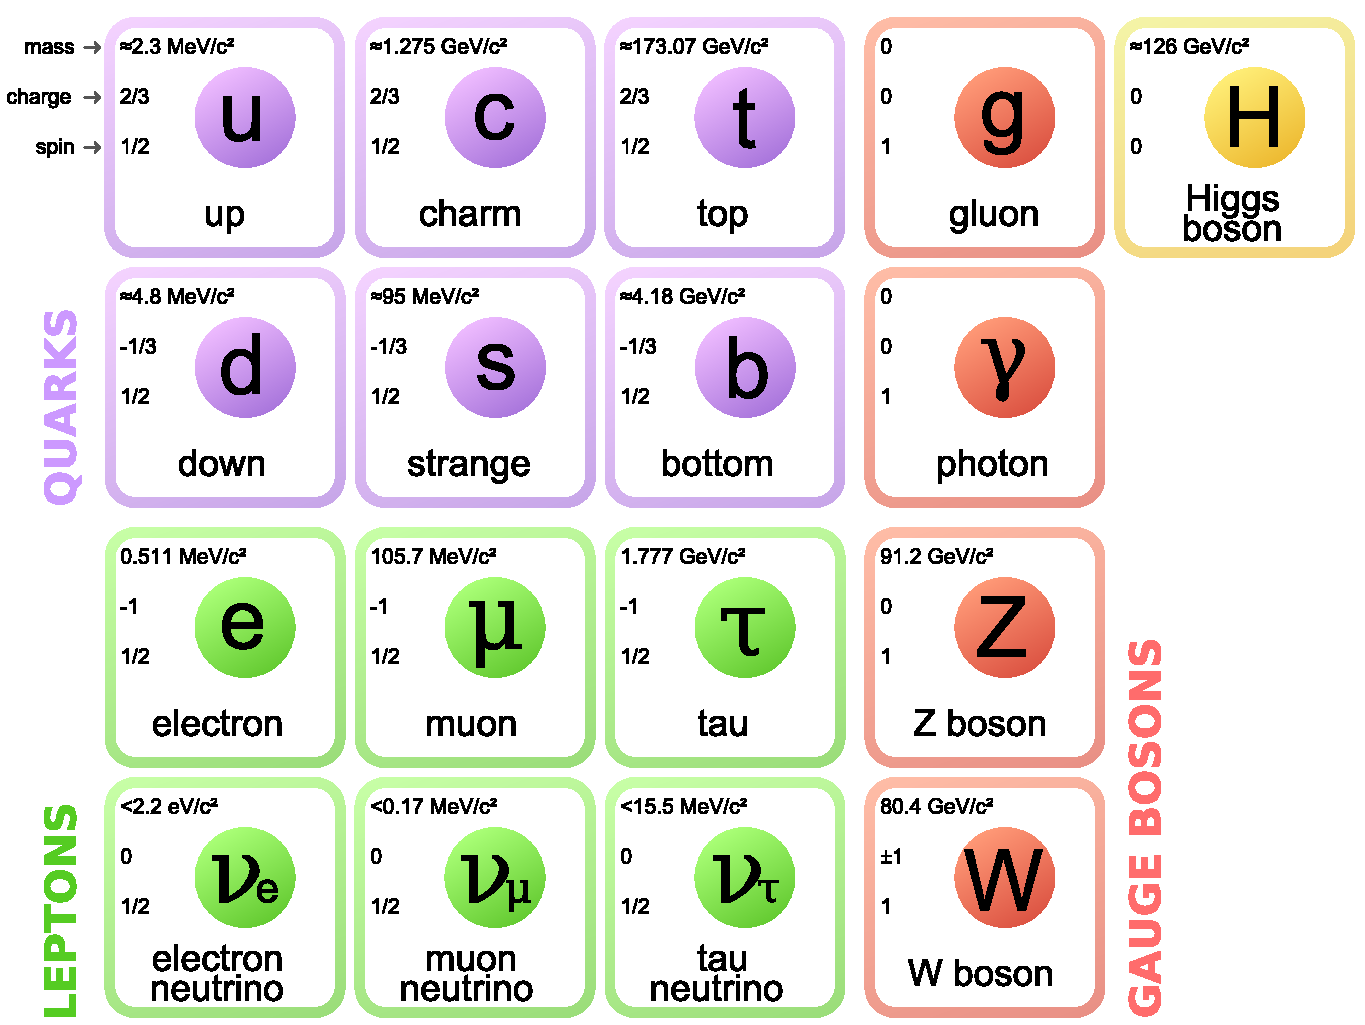
\includegraphics[width=\textwidth]{figures/standard_model.pdf}
    \caption{The particles of the standard model with information about their
        type, their mass, charge, and spin. The quarks and leptons make up
        matter, while the gauge bosons mediate interactions. The Higgs gives
        mass to the \W and \Z bosons.
        % https://en.wikipedia.org/wiki/Standard_Model#mediaviewer/File:Standard_Model_of_Elementary_Particles.svg
        % \TODO{Source}
    }

    \label{fig:standard_model}
\end{figure}

There are two types of particles in the standard model: fermions---with half
integer spin---and bosons---with integer spin. The fermions, which make up all
of the matter in the universe, are further subdivided into two groups, leptons
and quarks, while the bosons are divided into gaguge bosons and the Higgs.  The
various particles are show schematically in \FIG~\ref{fig:standard_model}.

Leptons have \spinhalf and have charge $q=-1 \text{ or } 1$ for the massive
leptons, or 0 for the neutrinos. They interact electromagnetically (if they
have a non-zero charge) and weakly. There are three generations of leptons and
each generation consists of a charged, massive lepton, and an uncharged, nearly
massless neutrino. The lightest of the charged lepton generations is the
electron, which is stable. The next two generations contain the muon and the
tau, which are unstable and eventually decay to electrons. The tau, being very
heavy, decays quickly, while the muon is stable long enough to escape a
particle detector. Massive leptons are important in particle detection as they
provide a very clean decay signature. Neutrinos are very difficult to detect in
particle detectors, and so their presence is inferred from the missing energy
in the vector sum of all particles in the collision. This analysis uses
electrons to make its measurement.

Quarks also have \spinhalf although, unlike the leptons, their charge is
fractional and so takes values of $q = 2/3 \text{ or } -1/3$. They interact
strongly, electromagnetically, and weakly. There are three generations of
quarks, with each successive generation having a higher mass constituents. The
first generation consists of the up and down (u and d) quarks. These quarks are
stable and make up protons and neutrons, as well as pions. The next generation
of quarks contains the charm and the strange (c and s). They form heavier
states that decay quickly like the \jpsi and kaons. The final generation
consist of the heavy bottom (b), and the exteriorly heavy top (t)---the most
massive particle in the standard model. Bottom quarks can form bound states,
but top quarks are so heavy they decay before any bound states can form.

Quarks carry color charge, of which there are three: red (r),
blue (b), and green (g). Strongly interacting objects obey confinement, which
means that only color neutral (colorless) states are allowed. Because of
confinement, quarks bind together into colorless composite particles. These
particles are called mesons---with two quarks (\qqbar)---and baryons---with
three quarks (\baryon). When an object containing quarks breaks up, the
individual colored fragments will create additional colored objects to maintain
their colorless state. This leads to the formation of ``jets'' which are sprays
of high energy particles that originate from one of these fragments as it tries
to maintain its colorless state.

Bosons are the second type of particle in the standard model. They are further
subdivided into gauge bosons---which mediate the three forces---and the Higgs
boson---which gives mass to the \W and \Z bosons.

The gauge boson that mediates the strong force is the gluon. Gluons interact
with objects that carry color, and are themselves carriers of color, allowing
gluons to interact not only with quarks but with other gluons. Gluons can have
any one of eight different possible color-anticolor superpositions that form a
color-octet. This number comes from the number of generators of \SUthree. Such
octets are not unique, but a commonly used definition is listed in
\TAB~\ref{table:gluon_color}.

\begin{table}[h]
\centering
\begin{center}
    \begin{tabular}{ c  c }
        $\left( \xxbar{r}{b} + \xxbar{b}{r} \right) / \sqrt{2}$ &
        $-i \left( \xxbar{r}{b} - \xxbar{b}{r} \right) / \sqrt{2}$ \\
        $\left( \xxbar{r}{g} + \xxbar{g}{r} \right) / \sqrt{2}$ &
        $-i \left( \xxbar{r}{g} - \xxbar{g}{r} \right) / \sqrt{2}$ \\
        $\left( \xxbar{b}{g} + \xxbar{g}{b} \right) / \sqrt{2}$ &
        $-i \left( \xxbar{b}{g} - \xxbar{g}{b} \right) / \sqrt{2}$ \\
        $\left( \xxbar{r}{r} - \xxbar{b}{b} \right) / \sqrt{2}$ &
        $\left( \xxbar{r}{r} - 2\xxbar{b}{b} + \xxbar{g}{g} \right) / \sqrt{6}$ \\
    \end{tabular}
    \caption{
        One of the possible color-octets. The colors are red ($r$), blue ($b$),
        green ($g$), and their anti-colors ($\overline{r}$, $\overline{b}$, and
        $\overline{g}$) .
    }
\label{table:gluon_color}
\end{center}
\end{table}

There are four gauge bosons that mediate the electroweak interaction: the photon
(\photon), the \Z, and the \Wpm. The photon and the \Z are uncharged, while the
\Wpm carries charge. The \W and \Z are not the particles described by the
\SUtwoUone group, but are instead linear combinations of these fields created
through combination with the Higgs mechanism. The \W participates in
interactions that change quark and lepton flavor, for example \ttoWb or
\mutoWnu.

The \Z boson acts as an excellent probe of precision physics as its well
measured mass (\Zmass) and its sharp width (\Zwidth) make it easy to identify
from its decay products \cite{pdg2014}. In a hadron collider the most common
\Ztoqq decay mode is difficult to select, and so \Ztoll decay modes are
preferred. In this analysis we look at the \Ztoee decay mode. A few common
decay modes and their branching fraction are listed in
\TAB~\ref{table:z_decays}.

\begin{table}[h]
\centering
\begin{center}
    \begin{tabular}{ l  r }
        Mode & Fraction $\left( \Gamma_{i} / \Gamma \right)$ \\ \hline
        $\Ztoqq$ & $69.91 \pm 0.06\%$ \\
        $\Ztoee$ & $3.363 \pm 0.004\%$ \\
        $\Ztomumu$ & $3.366 \pm 0.007\%$ \\
        $\Ztotautau$ & $3.370 \pm 0.008\%$ \\
        $\Ztonunu$ & $20.00 \pm 0.06\%$ \\
    \end{tabular}
    \caption{
        Selected decay modes of the \Z boson.
    }
\label{table:z_decays}
\end{center}
\end{table}
